\documentclass[a4paper,12pt]{report}
\usepackage[utf8]{inputenc} % To use Unicode (e.g. Turkish) characters
\renewcommand{\labelenumi}{(\roman{enumi})}
\usepackage{amsmath, amsthm, amssymb}
 % Some extra symbols
\usepackage[bottom]{footmisc}
\usepackage{cite}
\usepackage{url}
\usepackage{graphicx}
\usepackage{longtable}
\graphicspath{{figures/}} % Graphics will be here

\usepackage{multirow}
\usepackage{subfigure}
\usepackage{algorithm}
\usepackage{algorithmic}
\usepackage{float}
\usepackage{booktabs}

\usepackage{tikz}
\usetikzlibrary{arrows.meta,positioning}

\begin{document}

% Title Page
\title{CMPE 491 \\ Efficient QUBO formulations for Quantum Adiabatic Computation of The Steiner Tree Problem}
\author{
Dağhan Erdönmez \\
Advisor: \\ 
Hüseyin Birkan Yılmaz
}
\date{}
\maketitle{}

GitHub repository of the project can be accessed at: 
\begin{itemize}
    \item https://github.com/daghanerdonmez/finale
    \item https://github.com/daghanerdonmez/finale/wiki
\end{itemize}
\pagenumbering{roman}
\tableofcontents

\chapter{INTRODUCTION}
\pagenumbering{arabic}

\section{Broad Impact}

Efficient QUBO formulations are important for determining how well combinatorial optimization problems can be handled by quantum annealers and related binary optimization solvers. In problems such as the Steiner Tree Problem, the difficulty is not only to encode the objective correctly, but also to represent the feasibility structure of the problem in a way that penalizes invalid configurations. A formulation whose global minimum corresponds to the correct solution may still perform poorly in practice if many infeasible or structurally incorrect configurations have low energy.

The Steiner Tree Problem has applications in network design, routing, and infrastructure planning, where the goal is to connect a required set of nodes with minimum total cost. Studying QUBO formulations for this problem is useful both from an application perspective and from the broader perspective of quantum optimization, since it illustrates the trade-off between formulation compactness, constraint strength, interaction complexity, and solver performance.

More generally, this work contributes to understanding the practical limitations of QUBO-based optimization. In particular, it highlights issues such as infeasible-state penalization, large penalty coefficients, dense quadratic interactions, and sensitivity to formulation structure. These factors are central in evaluating the usefulness of QUBO formulations on quantum annealers, simulated quantum annealing methods, and classical binary quadratic optimization tools.

\section{Ethical Considerations}

This work is theoretical and computational in nature. It does not involve human subjects, personal data, or sensitive information, so there are no direct ethical concerns related to privacy, consent, or data security.

At the same time, optimization methods can ultimately be applied in domains such as logistics, communication networks, and infrastructure systems. Therefore, more effective optimization techniques may have broader social and economic consequences depending on how they are used. These concerns are not specific to the present study, but they motivate responsible interpretation and application of optimization results.

From a research perspective, the main ethical responsibilities are transparency, reproducibility, and proper attribution. We therefore present the formulations explicitly, compare them using clearly defined criteria, and distinguish our proposed formulation from prior work through appropriate citation and discussion.

\chapter{PROJECT DEFINITION AND PLANNING}

\section{Project Definition}

We study QUBO (Quadratic Unconstrained Binary Optimization) formulations for the Steiner Tree Problem (STP). The goal is not only to obtain a formulation whose minimizing configuration corresponds to the optimal Steiner tree, but also to construct a model in which infeasible configurations are properly penalized. This distinction is important because a QUBO formulation may encode the correct optimum while still assigning low energy to invalid graph structures, which can make the formulation ineffective in practice.

During the project, we examined several QUBO formulations for the STP. In addition to the general elementary formulation given by Lucas, we studied a recently proposed path-based formulation and an ordering-based formulation. The path-based formulation was found to be structurally insufficient, while the ordering-based formulation provides a much stronger reference model. However, the ordering-based model uses global ordering variables and contains a transitivity term that leads to cubic interaction complexity.

Motivated by this observation, we propose a depth-based directed-edge formulation for the STP. The formulation keeps the useful directed-edge structure of the ordering-based model, but replaces the all-pairs ordering variables with binary-encoded depth variables. This removes the global ordering-transitivity constraint and leads to improved asymptotic complexity, especially for sparse graphs. The proposed formulation is analyzed in terms of correctness, variable complexity, interaction complexity, coefficient ranges, and empirical solver behavior.

\section{Project Planning}

\subsection{Project Time and Resource Estimation}

The work was organized over several stages: literature review, formulation analysis, formulation development, implementation, experimentation, and reporting. The first stage focused on understanding existing QUBO and Ising formulations for combinatorial optimization problems, especially formulations related to network design and the Steiner Tree Problem. This included studying general QUBO construction techniques as well as STP-specific formulations.

The next stage consisted of analyzing existing formulations and identifying their strengths and weaknesses. In particular, we considered whether each formulation penalizes infeasible configurations sufficiently, how many binary variables it requires, and how many quadratic interactions it introduces. Based on this analysis, we developed the proposed depth-based formulation and compared it against the ordering-based formulation.

The implementation and experimentation stages consisted of coding the formulations, generating representative STP instances, constructing the corresponding binary quadratic models, and analyzing their size and solver behavior. The main resources required were a personal computer for development and simulation, access to the relevant literature, and Python-based optimization libraries such as \texttt{dimod}, \texttt{OpenJij}, and \texttt{Gurobi}. Although access to quantum annealing hardware would be useful for broader evaluation, it is not necessary for the core formulation and complexity analysis.

\subsection{Success Criteria}

We regard the study as successful if it satisfies the following goals:
\begin{itemize}
    \item identifying and comparing existing QUBO formulations for the Steiner Tree Problem,
    \item distinguishing formulations that merely encode the correct optimum from formulations that penalize infeasible configurations structurally,
    \item proposing a valid QUBO formulation for the STP based on directed edges and depth variables,
    \item comparing the proposed formulation with the ordering-based formulation in terms of binary variable complexity and quadratic interaction complexity,
    \item implementing the formulations and evaluating their empirical size, coefficient ranges, and solver behavior on representative STP instances.
\end{itemize}

\subsection{Risk Analysis}

A primary risk is that improving the structural validity of a QUBO formulation may require additional variables, auxiliary constraints, or large penalty coefficients. These additions can make the resulting binary quadratic model larger, denser, or numerically harder for solvers. Therefore, a formulation with better theoretical structure may not automatically lead to better practical solver performance.

Another risk is that solver behavior may obscure the actual quality of the formulation. Simulated quantum annealing and related sampling-based methods are sensitive to penalty coefficients, coefficient ranges, interaction density, and random sampling effects. For this reason, solver results must be interpreted together with structural validity checks and formulation-level complexity analysis.

There is also the risk that asymptotic improvements do not appear clearly on small benchmark instances. Since the proposed formulation is mainly motivated by reducing variable and interaction complexity, especially in sparse graphs, its advantages may become more visible as the instance size grows. We address these risks by comparing formulations both theoretically and experimentally, considering not only solution energy but also validity, model size, interaction count, and coefficient scale.

\chapter{RELATED WORK}

Quadratic Unconstrained Binary Optimization (QUBO) has become a standard framework for encoding combinatorial optimization problems for quantum annealing and related optimization approaches. Many NP-hard problems can be expressed in QUBO or Ising form, which makes it possible to study them within a common binary optimization framework and solve them using both quantum and classical methods.

Foundational work in this area includes the work of \cite{Lucas_2014}, which presents Ising formulations for many NP problems, including an elementary formulation of the Steiner Tree Problem. While this formulation is valuable as a general construction, it is not optimized for compactness and leads to unfavorable binary-variable and quadratic-interaction complexity. Similarly, \cite{glover2019tutorialformulatingusingqubo} provides practical guidance on constructing and using QUBO models, including the general penalty-based methodology used to convert constrained optimization problems into unconstrained binary objectives.

More recent work has also proposed STP-specific QUBO formulations. The path-based formulation of \cite{li2026steinertreeproblemnovel} attempts to model the Steiner Tree Problem by constructing paths from a root to the terminals. However, we found that this formulation does not fully enforce the required global Steiner-tree structure. In particular, its path-overlap condition is not sufficient to guarantee that the selected paths form one connected valid Steiner tree.

A stronger formulation is given by \cite{alex_2017}, which uses directed edge variables together with ordering variables. This ordering-based formulation is structurally more reliable, since it directly enforces parent relations and prevents cyclic or invalid directed structures through ordering constraints. However, the use of all-pairs ordering variables introduces a large number of binary variables, and the ordering-transitivity constraint leads to cubic interaction complexity.

Our work is motivated by this trade-off. Rather than using a purely elementary construction or a path-overlap formulation, we take the ordering-based formulation as the main reference point and develop a depth-based directed-edge formulation. The proposed formulation keeps the useful directed-edge and parent-constraint structure, but replaces global ordering variables with binary-encoded depth variables. This reduces the asymptotic complexity in sparse graphs while still aiming to penalize infeasible configurations structurally.

\chapter{METHODOLOGY}

\begin{figure}[htbp]
\centering
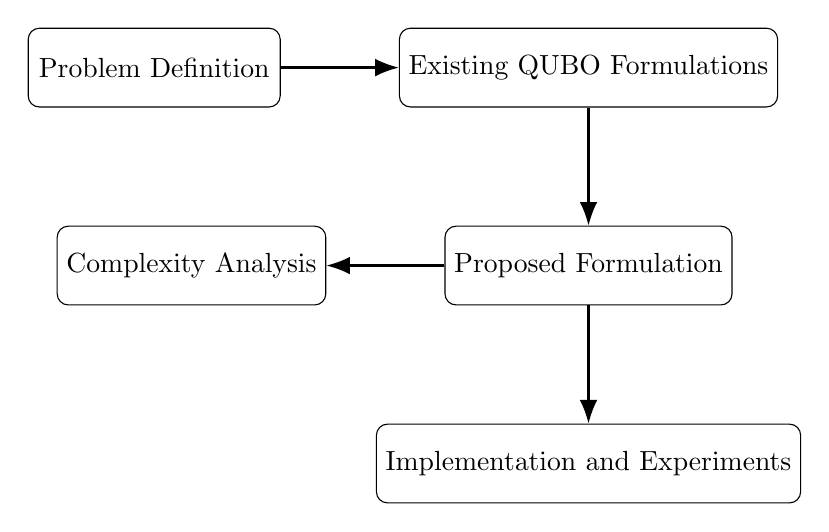
\begin{tikzpicture}[
node distance=1.5cm,
box/.style={draw, rectangle, rounded corners, minimum width=3.2cm, minimum height=1cm, align=center},
arrow/.style={-{Latex[length=3mm]}, thick}
]

\node[box] (problem) {Problem Definition};
\node[box, right=of problem] (review) {Existing QUBO Formulations};
\node[box, below=of review] (ours) {Proposed Formulation};
\node[box, left=of ours] (analysis) {Complexity Analysis};
\node[box, below=of ours] (experiments) {Implementation and Experiments};

\draw[arrow] (problem) -- (review);
\draw[arrow] (review) -- (ours);
\draw[arrow] (ours) -- (analysis);
\draw[arrow] (ours) -- (experiments);

\end{tikzpicture}
\caption{High-level workflow of the study.}
\label{fig:methodology_workflow}
\end{figure}

\section{Methodological Overview}

We study the Steiner Tree Problem through QUBO formulations designed for quantum annealing and related binary optimization methods. The methodology consists of four main parts. First, we define the Steiner Tree Problem and the general QUBO framework. Second, we examine existing QUBO formulations for the problem, with particular attention to whether they penalize infeasible configurations and how their variable and interaction counts scale. Third, we present our proposed formulation. Finally, we analyze and compare the formulations theoretically and experimentally.

A central point in this study is that a QUBO formulation should not only have the optimal solution as its minimizing configuration. It should also penalize infeasible configurations that do not correspond to valid Steiner trees. Otherwise, the energy landscape may contain many structurally invalid low-energy states, making the formulation difficult to solve in practice.

The proposed formulation is motivated by the ordering-based formulation of \cite{alex_2017}. The ordering-based model is structurally strong, but it uses all-pairs ordering variables and contains an ordering-transitivity term with cubic interaction complexity. Our formulation keeps the directed-edge and parent-constraint structure of this model, but replaces the all-pairs ordering variables with binary-encoded depth variables. This removes the global ordering-transitivity constraint and improves the asymptotic complexity in sparse graphs.

\section{QUBO Background}

\subsection{Quadratic Unconstrained Binary Optimization}

A QUBO problem is an optimization problem of the form
\[
\min_{x \in \{0,1\}^n} x^\top Q x,
\]
where \(Q\) is a real-valued matrix and the decision variables are binary. Equivalently, the objective can be written as
\[
\min
\left(
\sum_i h_i x_i
+
\sum_{i<j} J_{ij}x_i x_j
\right).
\]

Constrained combinatorial optimization problems are usually converted into QUBO form by adding penalty terms for constraint violations. A typical penalty-based Hamiltonian has the form
\[
H(x)
=
H_{\text{cost}}(x)
+
\lambda H_{\text{penalty}}(x),
\]
where \(H_{\text{cost}}\) represents the original objective and \(H_{\text{penalty}}\) is zero for feasible configurations and positive for infeasible configurations.

\subsection{Penalty-Based Formulation Strategy}

For an equality constraint
\[
g(x)=0,
\]
a standard QUBO penalty is
\[
g(x)^2.
\]
This term is zero exactly when the constraint is satisfied and positive otherwise. Therefore, a constrained objective
\[
\min f(x)
\quad \text{subject to} \quad
g_i(x)=0
\]
can be converted into
\[
H(x)
=
f(x)
+
\sum_i \lambda_i g_i(x)^2.
\]

For inequality constraints, slack variables are usually introduced to convert the inequality into an equality. Since QUBO variables must be binary, integer-valued variables and slack variables are represented using binary expansion.

\section{The Steiner Tree Problem}

Let
\[
G=(V,E)
\]
be a connected undirected graph with nonnegative edge weights \(c_{uv}\), and let
\[
T\subseteq V
\]
be the set of terminal vertices. The Steiner Tree Problem asks for a minimum-weight connected subgraph that spans all terminals. Vertices in \(V\setminus T\) may be included if doing so reduces the total cost; these vertices are called Steiner vertices.

We choose one terminal
\[
r\in T
\]
as the root. The goal is to select a set of edges that connects every terminal to the root while minimizing the total selected edge cost.

Throughout the report, we use the notation
\[
n=|V|,\qquad m=|E|,\qquad k=|T|.
\]

\section{Existing Ordering-Based Formulation}

The strongest existing formulation considered in this work is the ordering-based formulation of \cite{alex_2017}. This formulation uses directed edge variables and global ordering variables to enforce an arborescence-like structure.

\subsection{Variables}

For each undirected edge \(\{u,v\}\in E\), directed edge variables are introduced. If neither endpoint is the root, both directions are allowed:
\[
e_{uv}, e_{vu}\in\{0,1\}.
\]
For edges incident to the root \(r\), only the outward direction is used:
\[
e_{ru}\in\{0,1\}.
\]

The formulation also introduces ordering variables
\[
x_{uv}\in\{0,1\},
\qquad u,v\in V\setminus\{r\},\ u<v.
\]
These variables represent the relative order of non-root vertices.

The number of binary variables is
\[
N_{\text{vars}}^{\text{ord}}
=
(2m-d_r)
+
\binom{n-1}{2},
\]
where
\[
d_r=\deg(r).
\]
Therefore,
\[
N_{\text{vars}}^{\text{ord}}
=
\mathcal{O}(n^2).
\]

\subsection{Hamiltonian Structure}

The ordering-based formulation has the form
\[
H_{\text{ord}}(e,x)
=
P_I F_I(e,x)
+
O_I(e),
\]
where \(O_I(e)\) is the cost term and \(F_I(e,x)\) is the sum of constraint penalties.

The cost term is
\[
O_I(e)
=
\sum_{\substack{\{u,v\}\in E\\u,v\neq r}}
c_{uv}(e_{uv}+e_{vu})
+
\sum_{\{r,u\}\in E}
c_{ru}e_{ru}.
\]

Let
\[
c_{\max}=\max_{\{u,v\}\in E}c_{uv}.
\]
Fowler chooses the penalty weight and cut-off
\[
P_I=(n-1)c_{\max}+1,
\qquad
M_I=(n-1)c_{\max}.
\]

The penalty part consists of ordering consistency, edge-order consistency, terminal parent constraints, non-terminal parent constraints, and fake-root prevention:
\[
F_I(e,x)
=
F_{I,1}(x)
+
F_{I,2}(e,x)
+
F_{I,3}(e)
+
|V|F_{I,4}(e)
+
F_{I,5}(e).
\]

\subsection{Ordering Consistency}

The ordering consistency term enforces transitivity among the ordering variables:
\[
F_{I,1}(x)
=
\sum_{\substack{u<v<w\\u,v,w\neq r}}
\left(
x_{uw}
+
x_{uv}x_{vw}
-
x_{uv}x_{uw}
-
x_{uw}x_{vw}
\right).
\]

This term is responsible for the cubic interaction complexity of the ordering-based formulation, since it creates
\[
3\binom{n-1}{3}
\]
quadratic interactions. Hence,
\[
F_{I,1}
=
\mathcal{O}(n^3).
\]

\subsection{Edge-Order Consistency}

For every original non-root edge \(\{u,v\}\in E\), with \(u<v\), the selected direction must agree with the ordering bit:
\[
F_{I,2}(e,x)
=
\sum_{\substack{\{u,v\}\in E,\ u<v\\u,v\neq r}}
\left[
e_{uv}(1-x_{uv})
+
e_{vu}x_{uv}
\right].
\]
If \(x_{uv}=1\), the direction \(u\to v\) is allowed and \(v\to u\) is penalized; if \(x_{uv}=0\), the roles are reversed.

\subsection{Parent Constraints}

Each non-root terminal must have exactly one incoming selected edge:
\[
F_{I,3}(e)
=
\sum_{v\in T\setminus\{r\}}
\left(
1-\sum_{u:(u,v)\in A} e_{uv}
\right)^2.
\]

For non-terminal vertices, the formulation penalizes multiple parents:
\[
F_{I,4}(e)
=
\sum_{v\in V\setminus T}
\sum_{\substack{(u,v),(w,v)\in A\\u<w}}
e_{uv}e_{wv}.
\]
Equivalently, if \(q_v\) is the selected indegree of \(v\), then
\[
F_{I,4}(e)
=
\sum_{v\in V\setminus T}\binom{q_v}{2}.
\]
Fowler's displayed formula writes the inner pair sum compactly without an explicit \(u<w\) condition. His subsequent proof gives the binomial expression above, which confirms that the intended sum is over unordered distinct pairs of incoming arcs. Counting diagonal terms would incorrectly penalize a valid non-terminal with exactly one parent.

It also prevents a non-terminal from acting as a fake root:
\[
F_{I,5}(e)
=
\sum_{v\in V\setminus T}
\left(
1-\sum_{u:(u,v)\in A}e_{uv}
\right)
\left(
\sum_{w:(v,w)\in A}e_{vw}
\right).
\]

\subsection{Motivation for a New Formulation}

The ordering-based formulation is structurally strong because it directly enforces parent relations and uses ordering constraints to prevent cycles. However, the all-pairs ordering variables and the transitivity term introduce high complexity. In particular, its interaction complexity is dominated by
\[
\mathcal{O}(n^3).
\]

This motivates replacing global ordering variables with a more compact mechanism. Our formulation does this by using depth variables.

\section{Proposed Depth-Based Directed-Edge Formulation}

\subsection{Main Idea}

Our formulation keeps the directed-edge structure of the ordering-based formulation, but replaces all-pairs ordering variables with binary-encoded depth variables. Instead of explicitly storing the relative order of every pair of vertices, we assign a depth value to each vertex. If a directed edge \(u\to v\) is selected, then \(v\) must have greater depth than \(u\).

The main replacement is therefore
\[
x_{uv}
\quad \longrightarrow \quad
o_v.
\]

This removes the global ordering-transitivity term and replaces it with local depth-consistency constraints on selected directed edges.

\subsection{Variables}

The formulation uses the following binary and integer variables.

For each allowed directed edge \((u,v)\in A\),
\[
e_{uv}\in\{0,1\}
\]
indicates whether the directed edge \(u\to v\) is selected.

For each non-terminal vertex \(v\in V\setminus T\),
\[
p_v\in\{0,1\}
\]
indicates whether the non-terminal vertex \(v\) is used in the tree.

For each vertex \(v\in V\),
\[
o_v\in\mathbb{Z}_{\ge 0}
\]
denotes the depth of \(v\). Since the final QUBO model requires binary variables, each depth variable is encoded as
\[
o_v
=
\sum_{i=0}^{N-1}2^i o_{v,i},
\qquad
o_{v,i}\in\{0,1\},
\]
where
\[
N=\left\lceil \log_2 n \right\rceil.
\]

For each directed edge \((u,v)\in A\), a slack variable
\[
g_{uv}\ge 0
\]
is used to convert the depth inequality into an equality. It is also binary-encoded using \(\lceil\log_2{2n+1}\rceil\) bits.

\subsection{Objective Function}

The cost term minimizes the total weight of selected directed edges:
\[
H_{\text{cost}}
=
\sum_{\substack{\{u,v\}\in E\\u,v\neq r}}
c_{uv}(e_{uv}+e_{vu})
+
\sum_{\{r,u\}\in E}
c_{ru}e_{ru}.
\]

Equivalently, this objective assigns the undirected edge cost to whichever directed version of the edge is selected.

\subsection{Root Depth Constraint}

The root is fixed at depth zero:
\[
o_r=0.
\]
The corresponding Hamiltonian term is
\[
H_{\text{root}}
=
o_r^2.
\]

This gives a reference point for all other depth variables.

\subsection{Terminal Parent Constraint}

Each non-root terminal must have exactly one incoming edge:
\[
\sum_{u:(u,v)\in A} e_{uv}=1,
\qquad
v\in T\setminus\{r\}.
\]

The Hamiltonian term is
\[
H_3
=
\sum_{v\in T\setminus\{r\}}
\left(
1-\sum_{u:(u,v)\in A}e_{uv}
\right)^2.
\]

This ensures that every terminal other than the root is connected to the directed structure through one parent.

\subsection{Non-Terminal Parent and Usage Constraint}

For each non-terminal vertex, the usage variable \(p_v\) is linked to the number of incoming edges:
\[
p_v
=
\sum_{u:(u,v)\in A}e_{uv},
\qquad
v\in V\setminus T.
\]

The corresponding Hamiltonian term is
\[
H_4
=
\sum_{v\in V\setminus T}
\left(
p_v-\sum_{u:(u,v)\in A}e_{uv}
\right)^2.
\]

If \(p_v=0\), the vertex has no parent and is not used. If \(p_v=1\), the vertex has exactly one parent and is included in the selected directed structure.

\subsection{No Fake Non-Terminal Root Constraint}

A non-terminal vertex should not have outgoing selected edges unless it is itself used. Therefore, for each non-terminal \(v\in V\setminus T\), we penalize
\[
e_{vw}(1-p_v)
\]
for outgoing edges \((v,w)\in A\). The Hamiltonian term is
\[
H_5
=
\sum_{v\in V\setminus T}
\sum_{w:(v,w)\in A}
e_{vw}(1-p_v).
\]

This prevents unused non-terminal vertices from acting as artificial roots of disconnected directed components.

\subsection{Depth Consistency Constraint}

If a directed edge \(u\to v\) is selected, then \(v\) must be deeper than \(u\):
\[
e_{uv}=1
\implies
o_v\ge o_u+1.
\]

Using a sufficiently large constant \(M\), this implication is written as
\[
o_v
\ge
o_u+1-M(1-e_{uv}).
\]

Equivalently,
\[
o_v-o_u-1+M(1-e_{uv})\ge 0.
\]

Introducing a nonnegative slack variable \(g_{uv}\), we obtain
\[
o_v-o_u-1+M(1-e_{uv})-g_{uv}=0.
\]

The Hamiltonian term is
\[
H_{\text{depth}}
=
\sum_{(u,v)\in A}
\left(
o_v-o_u-1+M(1-e_{uv})-g_{uv}
\right)^2.
\]

When \(e_{uv}=1\), the constraint becomes
\[
o_v-o_u-1-g_{uv}=0,
\]
which implies
\[
o_v\ge o_u+1.
\]
Therefore, every selected directed edge must increase depth. This prevents directed cycles, because a directed cycle would require depth to strictly increase around a closed loop.

\subsection{Complete Hamiltonian}

The complete Hamiltonian of the proposed formulation is
\[
H_{\text{ours}}
=
H_{\text{cost}}
+
\lambda
\left(
H_{\text{root}}
+
H_{\text{depth}}
+
H_3
+
H_4
+
H_5
\right).
\]

Here, \(H_{\text{cost}}\) minimizes the total selected edge cost, while the remaining terms enforce the directed tree structure. The penalty coefficient \(\lambda>0\) is chosen sufficiently large so that violating the structural constraints is energetically unfavorable compared to reducing the edge cost.

\section{Variable Complexity}

Let
\[
d_r=\deg(r).
\]

The number of directed edge variables is
\[
2m-d_r,
\]
because both directions are allowed for non-root edges, while only the outgoing direction is used for edges incident to the root.

The number of depth variables is
\[
nN,
\]
where
\[
N=\left\lceil\log_2 n\right\rceil.
\]

The number of depth slack variables is
\[
(2m-d_r)N.
\]

The number of non-terminal usage variables is
\[
n-k.
\]

Therefore, the total number of binary variables in the proposed formulation is
\[
N_{\text{vars}}^{\text{ours}}
=
(2m-d_r)
+
nN
+
(2m-d_r)N
+
(n-k).
\]

Equivalently,
\[
N_{\text{vars}}^{\text{ours}}
=
(2m-d_r)(N+1)
+
nN
+
(n-k).
\]

Thus,
\[
N_{\text{vars}}^{\text{ours}}
=
\mathcal{O}(m\log n+n\log n).
\]

For connected sparse graphs where \(m=\mathcal{O}(n)\), this becomes
\[
N_{\text{vars}}^{\text{ours}}
=
\mathcal{O}(n\log n).
\]

\section{Interaction Complexity}

We count the number of quadratic interactions produced by each term of the Hamiltonian.

The cost term is linear, so it contributes no quadratic interactions:
\[
H_{\text{cost}}:\qquad 0.
\]

The root-depth term contains the square of a binary-encoded depth variable:
\[
H_{\text{root}}:\qquad \binom{N}{2}.
\]

For each directed edge \((u,v)\), the depth constraint contains the variables of \(o_u\), \(o_v\), the edge variable \(e_{uv}\), and the slack variable \(g_{uv}\). The number of variables inside each squared expression is
\[
3N+1.
\]
Therefore, the number of quadratic interactions from the depth constraints is
\[
H_{\text{depth}}:
\qquad
(2m-d_r)\binom{3N+1}{2}.
\]

For the terminal parent constraints, the number of interactions is
\[
H_3:
\qquad
\sum_{v\in T\setminus\{r\}}
\binom{\deg^-(v)}{2}.
\]

For the non-terminal parent and usage constraints, the variable \(p_v\) is included together with all incoming edge variables. Hence,
\[
H_4:
\qquad
\sum_{v\in V\setminus T}
\binom{\deg^-(v)+1}{2}.
\]

The no fake non-terminal root term contributes one interaction for each outgoing edge from each non-terminal:
\[
H_5:
\qquad
\sum_{v\in V\setminus T}\deg^+(v).
\]

Combining these terms, the total number of quadratic interactions is
\[
\begin{aligned}
N_{\text{quad}}^{\text{ours}}
={}&
\binom{N}{2}
+
(2m-d_r)\binom{3N+1}{2}
+
\sum_{v\in T\setminus\{r\}}
\binom{\deg^-(v)}{2}
\\
&+
\sum_{v\in V\setminus T}
\binom{\deg^-(v)+1}{2}
+
\sum_{v\in V\setminus T}\deg^+(v).
\end{aligned}
\]

Therefore,
\[
N_{\text{quad}}^{\text{ours}}
=
\mathcal{O}
\left(
mN^2+\sum_{v\in V}\deg(v)^2
\right).
\]

Since
\[
N=\mathcal{O}(\log n),
\]
we obtain
\[
N_{\text{quad}}^{\text{ours}}
=
\mathcal{O}
\left(
m\log^2 n+\sum_{v\in V}\deg(v)^2
\right).
\]

For sparse bounded-degree graphs,
\[
m=\mathcal{O}(n),
\qquad
\sum_{v\in V}\deg(v)^2=\mathcal{O}(n),
\]
so
\[
N_{\text{quad}}^{\text{ours}}
=
\mathcal{O}(n\log^2 n).
\]

\section{Comparison with the Ordering-Based Formulation}

The ordering-based formulation has
\[
N_{\text{vars}}^{\text{ord}}
=
(2m-d_r)+\binom{n-1}{2}
=
\mathcal{O}(n^2)
\]
binary variables.

Its interaction complexity is dominated by the ordering-transitivity term:
\[
3\binom{n-1}{3}
=
\mathcal{O}(n^3).
\]
Therefore,
\[
N_{\text{quad}}^{\text{ord}}
=
\mathcal{O}(n^3).
\]

In contrast, the proposed formulation has
\[
N_{\text{vars}}^{\text{ours}}
=
\mathcal{O}(m\log n+n\log n)
\]
variables and
\[
N_{\text{quad}}^{\text{ours}}
=
\mathcal{O}
\left(
m\log^2 n+\sum_{v\in V}\deg(v)^2
\right)
\]
quadratic interactions.

In sparse bounded-degree graphs, this gives
\[
N_{\text{vars}}^{\text{ours}}
=
\mathcal{O}(n\log n),
\qquad
N_{\text{quad}}^{\text{ours}}
=
\mathcal{O}(n\log^2 n),
\]
whereas the ordering-based formulation has
\[
N_{\text{vars}}^{\text{ord}}
=
\mathcal{O}(n^2),
\qquad
N_{\text{quad}}^{\text{ord}}
=
\mathcal{O}(n^3).
\]

Thus, the proposed formulation has a better asymptotic scaling than the ordering-based formulation for sparse graphs.

\section{Experimental Method}

After constructing the formulations, we implement them in Python and generate the corresponding binary quadratic models. The implementation allows the formulations to be compared in terms of binary variable count, quadratic interaction count, coefficient ranges, and solver behavior.

For each generated Steiner Tree instance, we construct the QUBO model and extract structural statistics such as the number of variables and interactions. We also solve the original Steiner Tree instance using an exact classical optimization method to obtain a reference optimum. This allows us to check whether the sampled QUBO solutions correspond to valid and optimal Steiner trees.

The QUBO models are solved using available binary quadratic optimization tools, including simulated quantum annealing through \texttt{OpenJij}. The returned samples are decoded into selected edges and checked for validity. In particular, we examine whether all terminals are connected, whether the selected edges form a valid tree-like structure, and whether the objective value matches the reference optimum.

The experimental evaluation therefore considers both theoretical and practical aspects of the formulations. The theoretical analysis focuses on asymptotic variable and interaction complexity, while the empirical analysis focuses on actual BQM size, coefficient scale, validity of returned solutions, and solver performance.

\chapter{REQUIREMENTS SPECIFICATION}

This work is research-oriented and does not target the development of an end-user software product. Therefore, it does not involve conventional functional or non-functional requirements, user interaction scenarios, or use case specifications. Instead, the main requirements arise from the mathematical modeling and experimental evaluation goals of the study.

At the formulation level, the model must represent the Steiner Tree Problem correctly as a QUBO. In particular, it must penalize infeasible configurations that do not correspond to valid Steiner-tree structures, rather than only ensuring that the global minimum is correct. The formulation must also remain compatible with QUBO solvers by using binary variables and quadratic objective terms.

At the comparison level, the project must allow different QUBO formulations for the Steiner Tree Problem to be evaluated using common criteria. These criteria include binary variable count, quadratic interaction count, asymptotic complexity, coefficient ranges, structural validity of decoded solutions, and empirical solver behavior.

At the implementation level, the system must support the construction of Steiner Tree instances, generation of the corresponding QUBO models, execution of solver runs, extraction of formulation statistics, and verification of the validity and optimality of the obtained solutions. For these reasons, this chapter is limited in scope compared to a standard software engineering project. The emphasis of the study is on mathematical formulation and empirical evaluation rather than on user-facing system requirements.

\chapter{DESIGN}

\section{Information Structure}

Although the study does not involve database design or persistent information storage, it still has a clear internal information structure. Each Steiner Tree instance is represented by a graph \(G=(V,E)\), a set of terminals \(T\), a designated root terminal \(r\), and edge weights \(c_e\). From this representation, the formulation introduces directed edge variables, non-terminal usage variables, binary-encoded depth variables, and slack variables required by the depth constraints.

The experimental data produced by the study also follows a structured form. For each problem instance, we store or compute the generated formulation, the corresponding binary quadratic model, the number of binary variables, the number of quadratic interactions, coefficient ranges, solver outputs, decoded selected edges, and post-processed validity checks. Thus, while a formal data model such as an ER diagram is unnecessary, the project still relies on a well-defined representation of instances, variables, formulations, and results.

\section{Information Flow}

The information flow of the study follows a simple but well-defined sequence. First, a Steiner Tree instance is generated or provided as input. This instance is then converted into one or more mathematical QUBO formulations. Each formulation is transformed into a binary quadratic model by assembling its objective and penalty terms. The resulting model is then analyzed directly and, when needed, passed to a solver.

After solving, the returned sample is decoded back into selected directed edges and corresponding undirected edges. The decoded solution is analyzed to determine both its objective value and its structural validity. In particular, we check whether all terminals are connected, whether the selected edges form a valid tree-like structure, and whether the objective value matches the reference optimum.

This flow of information can be summarized as:
\[
\begin{aligned}
\text{STP instance}
&\rightarrow \text{QUBO formulation}
\rightarrow \text{BQM construction}
\\
&\rightarrow \text{solver output}
\rightarrow \text{decoded solution}
\\
&\rightarrow \text{validity and complexity analysis}.
\end{aligned}
\]

\section{System Design}

The implementation is not intended as a deployable software product, but it still has a modular structure at the level of experimental design. One part of the code represents Steiner Tree instances and related graph data. Another part constructs QUBO models by assembling the objective and penalty terms of each formulation. Additional components handle solver execution, decoding of returned samples, validation of the resulting solutions, and extraction of statistics such as variable counts, interaction counts, and coefficient ranges.

This modular organization is useful because it separates formulation logic from experimentation and analysis. As a result, different formulations can be tested within the same general pipeline, and their theoretical and empirical properties can be compared consistently. Therefore, while the project does not require a full software architecture in the traditional sense, it does involve a clear internal design that supports formulation development and comparative evaluation.


\chapter{IMPLEMENTATION AND TESTING}

\section{Implementation}

The formulations are implemented in Python using QUBO-oriented tools such as \texttt{dimod} and \texttt{OpenJij}. The implementation represents Steiner Tree instances as weighted graphs with a specified terminal set and a chosen root terminal. From each instance, the code constructs the corresponding binary quadratic model by adding the objective and penalty terms of the formulation.

The implementation is organized around the Hamiltonian components of each formulation. Separate functions are used to add the cost term, parent constraints, root-depth constraint, depth-consistency constraints, and non-terminal usage constraints. This modular structure makes it possible to construct different formulations within the same experimental pipeline and compare their properties consistently.

In addition to model construction, the implementation includes routines for generating or loading problem instances, extracting binary variable counts, extracting quadratic interaction counts, recording coefficient ranges, and decoding solver outputs back into selected directed and undirected edges. The decoded solutions are then checked for structural validity and compared with reference solutions obtained by exact classical optimization methods.

\section{Testing}

Testing is carried out by applying the implemented formulations to multiple Steiner Tree instances and comparing the resulting QUBO models and solver outputs. The evaluation is not based only on whether the minimum-energy solution has low objective value. We also check whether the decoded solution forms a valid Steiner tree, whether all terminals are connected, and whether the selected edge set matches the reference optimum.

The formulations are compared using both theoretical and empirical criteria. The theoretical comparison focuses on binary variable complexity and quadratic interaction complexity. The empirical comparison records the actual number of variables, number of interactions, and coefficient ranges produced for generated benchmark instances. These quantities are important because QUBO solver performance is affected not only by the number of variables, but also by interaction density and coefficient scale.

Solver-based testing is performed using available binary quadratic optimization tools, including simulated quantum annealing through \texttt{OpenJij}. The returned samples are decoded and validated structurally. This allows us to observe whether the formulation produces valid low-energy configurations in practice and how sensitive the results are to the penalty coefficient.

\begin{figure}[htbp]
\centering
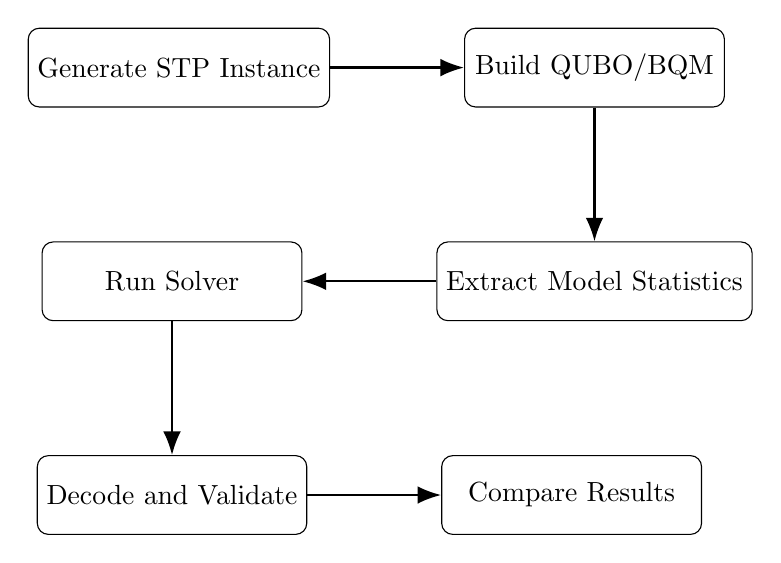
\begin{tikzpicture}[
node distance=1.7cm,
box/.style={draw, rectangle, rounded corners, minimum width=3.3cm, minimum height=1cm, align=center},
arrow/.style={-{Latex[length=3mm]}, thick}
]

\node[box] (instance) {Generate STP Instance};
\node[box, right=of instance] (build) {Build QUBO/BQM};
\node[box, below=of build] (stats) {Extract Model Statistics};
\node[box, left=of stats] (solve) {Run Solver};
\node[box, below=of solve] (check) {Decode and Validate};
\node[box, right=of check] (compare) {Compare Results};

\draw[arrow] (instance) -- (build);
\draw[arrow] (build) -- (stats);
\draw[arrow] (stats) -- (solve);
\draw[arrow] (solve) -- (check);
\draw[arrow] (check) -- (compare);

\end{tikzpicture}
\caption{Experimental procedure used to evaluate the formulations.}
\label{fig:experimental_workflow}
\end{figure}

\section{Deployment}

Not applicable. The project is research-oriented and does not involve deployment as a standalone software system.

\chapter{RESULTS}

\section{Overview}

In this chapter, we compare the proposed depth-based directed-edge formulation with the ordering-based formulation of \cite{alex_2017}. The comparison is carried out in two ways. First, we compare the formulations theoretically in terms of binary variable complexity and quadratic interaction complexity. Second, we compare their empirical behavior using benchmark instances solved with QUBO solvers and checked against exact ILP optima.

The main theoretical result is that the proposed formulation has better asymptotic complexity in sparse graphs. This improvement comes from replacing the all-pairs ordering variables of the ordering-based formulation with binary-encoded depth variables. As a result, the global ordering-transitivity term, which is responsible for cubic interaction complexity, is removed.

However, the empirical results show that better asymptotic complexity does not automatically imply better solver performance on the tested instances. In the current benchmarks, the ordering-based formulation performs better than the proposed formulation. This appears to be related to coefficient scaling and penalty dominance in the proposed formulation.

\section{Theoretical Complexity Comparison}

Let
\[
n=|V|,\qquad m=|E|,\qquad k=|T|,
\]
and let
\[
N=\left\lceil \log_2 n \right\rceil.
\]

The ordering-based formulation uses
\[
N_{\text{vars}}^{\text{ord}}
=
(2m-d_r)+\binom{n-1}{2}
\]
binary variables. Therefore,
\[
N_{\text{vars}}^{\text{ord}}
=
\mathcal{O}(n^2).
\]

Its interaction complexity is dominated by the ordering-transitivity term, which contributes
\[
3\binom{n-1}{3}
\]
quadratic interactions. Hence,
\[
N_{\text{quad}}^{\text{ord}}
=
\mathcal{O}(n^3).
\]

For the proposed formulation, the number of binary variables is
\[
N_{\text{vars}}^{\text{ours}}
=
(2m-d_r)(N+1)+nN+(n-k).
\]

Thus,
\[
N_{\text{vars}}^{\text{ours}}
=
\mathcal{O}(m\log n+n\log n).
\]

The number of quadratic interactions is
\[
N_{\text{quad}}^{\text{ours}}
=
\mathcal{O}
\left(
m\log^2 n+\sum_{v\in V}\deg(v)^2
\right).
\]

For sparse bounded-degree graphs, where
\[
m=\mathcal{O}(n),
\qquad
\sum_{v\in V}\deg(v)^2=\mathcal{O}(n),
\]
the proposed formulation satisfies
\[
N_{\text{vars}}^{\text{ours}}
=
\mathcal{O}(n\log n),
\]
and
\[
N_{\text{quad}}^{\text{ours}}
=
\mathcal{O}(n\log^2 n).
\]

Therefore, under sparse graph assumptions, the proposed formulation improves over the ordering-based formulation, whose variable and interaction complexities are
\[
\mathcal{O}(n^2)
\quad \text{and} \quad
\mathcal{O}(n^3),
\]
respectively.

\begin{figure}[htbp]
\centering
\includegraphics[width=1\linewidth]{sparse_160_2.png}
\caption{Comparison of variable and interaction counts for the ordering-based formulation and the proposed formulation (labeled as "hybrid") in sparse graph instances.}
\label{fig:sparse_complexity}
\end{figure}

\begin{figure}[htbp]
\centering
\includegraphics[width=1\linewidth]{dense_160_2.png}
\caption{Comparison of variable and interaction counts for the ordering-based formulation and the proposed formulation (labeled as "hybrid") in dense graph instances.}
\label{fig:dense_complexity}
\end{figure}

\section{Empirical Benchmark Setup}

We also evaluated the formulations experimentally on generated Steiner Tree instances. Two graph-generation settings were used. The first setting consists of sparse random graphs with edge probabilities
\[
p\in\{0.1,0.3,0.6\}.
\]
The second setting consists of geometric \(k\)-nearest-neighbor graphs with
\[
\text{knn}\in\{3,5,8\}.
\]

For both settings, the tested node counts were
\[
n\in\{4,6,8,10,12\},
\]
and the terminal counts were
\[
k\in\{2,3,4,5,6\}.
\]
Invalid parameter combinations with \(k>n\) were ignored. In total, the benchmark set contained 690 instances.

Each QUBO model was solved with a budget of 1000 reads, organized as 10 trials with 100 reads each. The QUBO results were compared against the exact optimum obtained from an ILP formulation. For each model and instance group, we measured success rate, first-hit reads, approximation ratio, feasible-read rate, and time to solution.

\section{Benchmark Results}

The benchmark results show that the ordering-based formulation performs better than the proposed formulation on the tested instances. In particular, the ordering-based formulation more frequently finds the ILP-optimal Steiner tree within the given read budget and produces a higher fraction of feasible decoded samples.

The proposed formulation does not show the expected practical advantage in these experiments, even though it has better sparse-graph asymptotic complexity. This indicates that the number of variables and interactions is not the only factor determining QUBO solver performance.

Manual experiments on larger instances also showed a similar pattern. The ordering-based formulation often produced feasible solutions close to the optimum, while the proposed formulation struggled to produce penalty-free feasible configurations. This suggests that the practical difficulty is not only caused by the small size of the benchmark instances.

\begin{figure}[H]
\centering
\includegraphics[width=0.9\linewidth]{succ.png}
\caption{Success rate of the ordering-based formulation and the proposed formulation across benchmark instances. Success rate is the fraction of instances for which the ILP-optimal Steiner tree was found within the 1000-read budget.}
\label{fig:success_rate}
\end{figure}

\begin{figure}[H]
\centering
\includegraphics[width=0.9\linewidth]{mfhr.png}
\caption{Mean first-hit reads for solved benchmark instances. This metric measures the average number of reads required before the ILP-optimal solution is first found, among instances where the optimum is found. Lower values indicate faster discovery of the optimum.}
\label{fig:first_hit_reads}
\end{figure}

\begin{figure}[H]
\centering
\includegraphics[width=0.9\linewidth]{mar.png}
\caption{Mean approximation ratio across benchmark instances. The approximation ratio is computed as the best cost found divided by the ILP-optimal cost. A value of \(1.0\) indicates that the optimal Steiner tree was found.}
\label{fig:approximation_ratio}
\end{figure}

\begin{figure}[H]
\centering
\includegraphics[width=0.9\linewidth]{frr.png}
\caption{Feasible-read rate across benchmark instances. This metric is the fraction of individual reads that decode to valid Steiner trees, meaning connected, acyclic, and spanning all terminals.}
\label{fig:feasible_read_rate}
\end{figure}

\begin{figure}[H]
\centering
\includegraphics[width=0.9\linewidth]{mtts.png}
\caption{Mean time to solution across benchmark instances. For solved instances, this is the wall-clock time until the optimum is first found. For unsolved instances, the full elapsed time for the read budget is used.}
\label{fig:time_to_solution}
\end{figure}

\section{Coefficient Scaling Issue}

To understand the poor empirical behavior of the proposed formulation, we examined the coefficient ranges of the generated Hamiltonians. Although the variable and interaction counts were not excessively large, the linear and quadratic coefficients in the proposed formulation were much larger than those of the ordering-based formulation.

A likely source of this issue is the depth-consistency penalty
\[
\left(
o_v-o_u-1+M(1-e_{uv})-g_{uv}
\right)^2.
\]
Here, \(M\) is proportional to the number of nodes. When this expression is squared, terms with coefficients proportional to \(M^2\) appear. Since the depth variables are also binary-expanded, additional factors of \(2^b\) appear in the coefficients. After multiplication by the penalty coefficient \(\lambda\), this can lead to very large linear and quadratic terms.

This creates a practical issue for the energy landscape. The actual objective coefficients, corresponding to edge costs, are relatively small compared to the penalty coefficients. As a result, the cost function can become dominated by large penalty terms, and the optimization objective may effectively become difficult for the solver to resolve.

\begin{table}[htbp]
\centering
\begin{tabular}{lrr}
\toprule
\textbf{Metric} & \textbf{Ordering-based} & \textbf{Proposed} \\
\midrule
Number of variables & 279 & 871 \\
Number of interactions & 3724 & 11882 \\
$\min(h_j)$ & $-447.0$ & $-2084160.0$ \\
$\max(h_j)$ & $8517.0$ & $2164320.0$ \\
$\min(J_{ij})$ & $-1002.0$ & $-513024.0$ \\
$\max(J_{ij})$ & $10020.0$ & $2052096.0$ \\
\bottomrule
\end{tabular}
\caption{Coefficient ranges for a representative benchmark instance. The proposed formulation has substantially larger coefficient magnitudes, mainly due to the big-\(M\) depth-consistency penalties.}
\label{tab:coefficient_ranges}
\end{table}

\section{Discussion}

The results show a distinction between theoretical formulation size and practical solver performance. The proposed formulation improves the asymptotic variable and interaction complexity in sparse graphs, but the current implementation introduces large coefficients through the depth penalties. This can make the resulting QUBO difficult to solve in practice.

Therefore, the proposed formulation should be viewed as a theoretically promising formulation whose practical performance still requires improvement. In particular, future work should focus on penalty scaling, coefficient normalization, and alternative depth encodings or constraint constructions that preserve the sparse-graph complexity advantage while reducing coefficient magnitudes.

\chapter{CONCLUSION}

In this project, we studied QUBO formulations for the Steiner Tree Problem. The main goal was not only to obtain a formulation whose global minimum corresponds to the optimal Steiner tree, but also to construct a formulation that penalizes infeasible configurations structurally.

We first examined existing QUBO formulations for the Steiner Tree Problem. Lucas's elementary formulation provides a general construction but has unfavorable complexity. The path-based formulation of Li et al. was found to be structurally insufficient because its path-overlap condition does not fully guarantee a valid connected Steiner tree. The ordering-based formulation of Fowler provides a much stronger reference model, but it uses all-pairs ordering variables and contains a cubic ordering-transitivity term.

Motivated by this limitation, we proposed a depth-based directed-edge formulation. The formulation keeps the useful directed-edge and parent-constraint structure of the ordering-based model, but replaces global ordering variables with binary-encoded depth variables. A selected directed edge is required to increase depth, which prevents directed cycles without requiring all-pairs ordering constraints.

The proposed formulation has
\[
N_{\text{vars}}^{\text{ours}}
=
\mathcal{O}(m\log n+n\log n)
\]
binary variables and
\[
N_{\text{quad}}^{\text{ours}}
=
\mathcal{O}
\left(
m\log^2 n+\sum_{v\in V}\deg(v)^2
\right)
\]
quadratic interactions. In sparse bounded-degree graphs, this becomes
\[
\mathcal{O}(n\log n)
\]
variables and
\[
\mathcal{O}(n\log^2 n)
\]
interactions. This improves over the ordering-based formulation, which has
\[
\mathcal{O}(n^2)
\]
variables and
\[
\mathcal{O}(n^3)
\]
interactions.

Empirically, however, the ordering-based formulation performed better in the current benchmarks. The proposed formulation often struggled to produce feasible low-energy samples. By examining the generated QUBO coefficients, we observed that the proposed formulation can produce large linear and quadratic coefficients, mainly due to the big-\(M\) depth-consistency constraints and binary expansion of depth variables.

Overall, the project produced a theoretically promising QUBO formulation for the Steiner Tree Problem, especially for sparse graphs, but also revealed an important practical limitation. The next stage of the project will focus on improving the coefficient scaling of the proposed formulation, tuning penalty coefficients more carefully, and exploring alternative encodings that preserve the asymptotic advantage while improving empirical solver behavior.

\bibliographystyle{unsrt}
\bibliography{references}


\end{document}
